\chapter{Experimentos e Resultados}
\label{cap:resultados}

Este capítulo relata a execução prática da metodologia descrita no Capítulo~\ref{chap:metodologia-avaliacao}, apresenta as restrições operacionais encontradas durante o processamento em nuvem e analisa os resultados comparativos das quatro configurações: \textbf{E1 (fragmentos)}, \textbf{E2 (páginas)}, \textbf{E3 (EDGAR sem visão)} e \textbf{E4 (EDGAR completo)}.

\section{Execução experimental e restrições operacionais}
\label{sec:execucao-e-restricoes}

Durante a execução do fluxo de ingestão na plataforma Modal, limites de cota e créditos computacionais para uso das GPUs NVIDIA T4 impediram o processamento integral do corpus planejado. Os livros de Cálculo, Teoria dos Grafos e Física foram processados por completo, mas o livro de Estatística precisou ser interrompido após o processamento parcial de suas páginas iniciais. Em razão desse corte, três perguntas de teste de Estatística cujas páginas de referência não haviam sido processadas foram retiradas antes da avaliação, por verificação direta da página-alvo no gabarito. A Tabela~\ref{tab:corpus-edgar} sintetiza o volume planejado e o efetivamente executado.

\begin{table}[H]
    \centering
    \caption{Relação entre páginas e perguntas planejadas na metodologia e efetivamente executadas.}
    \label{tab:corpus-edgar}
    {\ABNTEXfontereduzida
    \begin{tabular}{lrrrr}
        \toprule
        \textbf{Documento} &
        \shortstack{\textbf{Páginas}\\\textbf{planejadas}} &
        \shortstack{\textbf{Páginas}\\\textbf{processadas}} &
        \shortstack{\textbf{Perguntas}\\\textbf{planejadas}} &
        \shortstack{\textbf{Perguntas}\\\textbf{avaliadas}} \\
        \midrule
        Cálculo     & 218 & 218 & 6 & 6 \\
        Grafos      & 104 & 104 & 6 & 6 \\
        Física      & 152 & 152 & 6 & 6 \\
        Estatística & 104 &  26 & 6 & 3 \\
        \midrule
        \textbf{Total} & \textbf{578} & \textbf{500} & \textbf{24} & \textbf{21} \\
        \bottomrule
    \end{tabular}
    }
    \legend{Fonte: Elaborado pelo autor.}
\end{table}

Das 500 páginas processadas, 493 continham conteúdo útil para indexação (as sete restantes eram páginas divisórias ou continham apenas cabeçalhos e rodapés). Sobre essas 493 páginas, a indexação gerou \textbf{1.175 registros em E1 (fragmentos)}, \textbf{493 em E2 (páginas)}, \textbf{5.855 em E3 (EDGAR sem visão)} e \textbf{6.223 em E4 (EDGAR completo)}. Os 368 registros adicionais de E4 em relação a E3 correspondem a figuras e tabelas sem texto extraível que passaram a ser pesquisáveis por meio das descrições geradas pelo modelo Qwen3-VL-4B-Instruct.

As 21 perguntas avaliadas distribuem-se nas cinco categorias definidas na metodologia: sete de evidência visual, seis de raciocínio multimodal, três de recuperação de texto, três de fórmulas e duas de tabelas. Na etapa de geração, foram avaliadas 84 respostas (21 por configuração). Sob o orçamento comum de 5.000 unidades de entrada, cada prompt comportou de 1 a 3 páginas inteiras em E2, de 3 a 5 fragmentos em E1 e de 5 a 20 componentes em E3 e E4.

\section{Resultados comparativos}
\label{sec:resultados-comparativos}

Os resultados a seguir descrevem o comportamento observado nas 21 consultas avaliadas. Como a amostra é reduzida, pequenas diferenças entre as configurações indicam tendências do conjunto estudado, sem configurar prova de superioridade estatística geral.

\subsection{Recuperação de evidências}
\label{sec:resultados-recuperacao}

A Figura~\ref{fig:recuperacao-edgar} compara a capacidade de cada configuração para posicionar a página esperada do livro entre as cinco primeiras colocações da busca (\textit{Hit@5}) e a proximidade média dessa página em relação ao topo do ranking (\textit{MRR@5}).

\begin{figure}[H]
    \centering
    \caption{Comparação da recuperação de páginas entre as quatro configurações nas 21 perguntas.}
    \label{fig:recuperacao-edgar}
    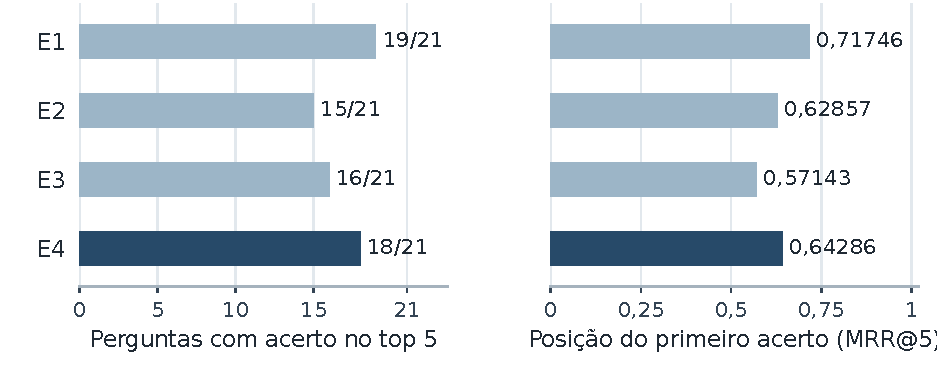
\includegraphics[width=\textwidth]{figuras/edgar-recuperacao-comparativa.pdf}
    \legend{Fonte: Elaborado pelo autor.}
\end{figure}

Observa-se na Figura~\ref{fig:recuperacao-edgar} que E1 (fragmentos) alcançou o maior número global de páginas corretas no topo (\textit{Hit@5} de 19/21 e \textit{MRR@5} de 0,72), seguida de perto por E4 (EDGAR completo), com 18/21 acertos e \textit{MRR@5} de 0,64. As configurações E3 (EDGAR sem visão) e E2 (páginas) obtiveram, respectivamente, 16/21 (\textit{MRR@5} de 0,57) e 15/21 (\textit{MRR@5} de 0,63). Quando a janela de busca foi ampliada para 128 páginas (\textit{Coverage@128}), todas as quatro configurações localizaram a página esperada nas 21 consultas.

A comparação direta entre E3 e E4 mostra onde o enriquecimento visual atua na busca: os dois acertos adicionais de E4 no \textit{Hit@5} ocorreram exatamente nas perguntas da categoria de \textbf{evidência visual} (na qual o acerto subiu de 3 em 7 consultas em E3 para 5 em 7 em E4). Além disso, nas seis consultas de \textbf{raciocínio multimodal}, embora todas as configurações tenham encontrado a página correta entre as cinco primeiras, a segmentação por componentes de E3 e E4 posicionou a página mais próxima do primeiro lugar (\textit{MRR@5} de 0,81, contra 0,67 em E1).

\subsection{Qualidade das respostas geradas}
\label{sec:qualidade-respostas}

Embora E1 tenha localizado uma página a mais que E4 nas cinco primeiras posições da busca, a avaliação das respostas geradas revelou o resultado inverso: \textbf{E4 (EDGAR completo) obteve a maior média nos três critérios de qualidade (correção factual, fundamentação e completude), somando 5,24 de 6 pontos possíveis, além de registrar o menor índice de alucinações (apenas 1 em 21 respostas)}. A Tabela~\ref{tab:rubrica-comparativa} e a Figura~\ref{fig:qualidade-edgar} resumem as notas obtidas por cada configuração.

\begin{table}[H]
    \centering
    \caption{Médias da avaliação por critérios de qualidade das respostas (n = 21 por configuração).}
    \label{tab:rubrica-comparativa}
    {\ABNTEXfontereduzida
    \begin{tabular}{@{}lccccc@{}}
        \toprule
        \textbf{Configuração} &
        \shortstack{\textbf{Correção}\\\textbf{factual (/2)}} &
        \shortstack{\textbf{Fundamen-}\\\textbf{tação (/2)}} &
        \shortstack{\textbf{Comple-}\\\textbf{tude (/2)}} &
        \shortstack{\textbf{Nota total}\\\textbf{média (/6)}} &
        \shortstack{\textbf{Alucina-}\\\textbf{ções}} \\
        \midrule
        E1 (fragmentos)      & 1,52 & 1,76 & 1,48 & \textbf{4,76} & 2/21 \\
        E2 (páginas)         & 1,29 & 1,48 & 1,29 & \textbf{4,05} & 5/21 \\
        E3 (EDGAR sem visão) & 1,43 & 1,62 & 1,33 & \textbf{4,38} & 2/21 \\
        E4 (EDGAR completo)  & \textbf{1,71} & \textbf{1,95} & \textbf{1,57} & \textbf{5,24} & \textbf{1/21} \\
        \bottomrule
    \end{tabular}
    }
    \legend{Fonte: Elaborado pelo autor.}
\end{table}

\begin{figure}[H]
    \centering
    \caption{Composição da nota média de qualidade das respostas por configuração.}
    \label{fig:qualidade-edgar}
    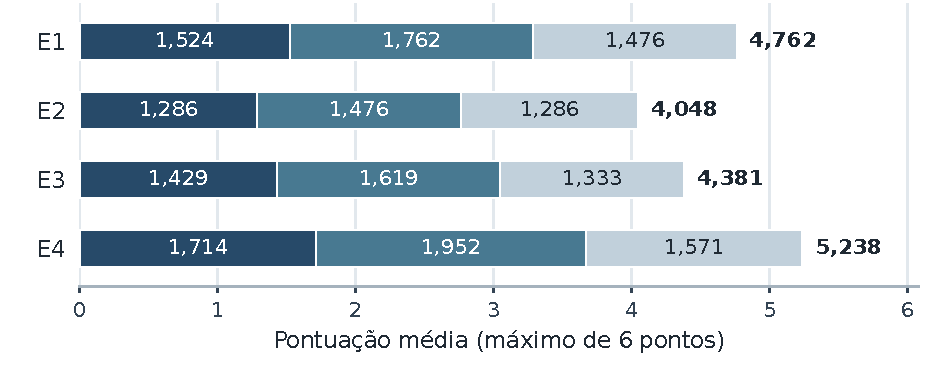
\includegraphics[width=\textwidth]{figuras/edgar-qualidade-comparativa.pdf}\par
    {\footnotesize
    \textcolor[HTML]{274A69}{\rule{0.8em}{0.8em}}~Correção factual \quad
    \textcolor[HTML]{487991}{\rule{0.8em}{0.8em}}~Fundamentação \quad
    \textcolor[HTML]{C1D0DB}{\rule{0.8em}{0.8em}}~Completude\par}
    \legend{Fonte: Elaborado pelo autor.}
\end{figure}

Dois fatores explicam a vantagem de E4 na qualidade final das respostas:
\begin{enumerate}
    \item \textbf{Ganhos expressivos em perguntas visuais e multimodais:} nas sete perguntas de evidência visual, a nota média saltou de 2,29/6 em E3 (sem visão) e 4,00/6 em E1 para \textbf{4,86/6 em E4}, eliminando as alucinações nessa categoria. Nas seis perguntas de raciocínio multimodal, a combinação de componentes enxutos no contexto levou E4 a \textbf{5,67/6} (e E3 a 5,50/6), superando os fragmentos de E1 (4,33/6) e as páginas inteiras de E2 (4,67/6), que ocupam o orçamento de entrada com muito texto periférico.
    \item \textbf{Limitação pontual em fórmulas isoladas:} nas consultas de texto corrido e de tabelas, todas as configurações tiveram desempenho elevado e semelhante. Já nas três perguntas sobre fórmulas matemáticas isoladas, E1 obteve média superior a E4 (5,33/6 contra 4,33/6), pois blocos contínuos de 1.000 caracteres preservam as frases ao redor da equação, enquanto o EDGAR não cria registros independentes para fórmulas isoladas.
\end{enumerate}

\subsection{Resultados da avaliação com RAGAS}
\label{sec:resultados-ragas}

Como avaliação complementar automatizada, foram calculadas as cinco métricas do \textit{framework} RAGAS 0.4.3. Das 420 avaliações previstas, 373 geraram notas válidas e 47 foram interrompidas porque a saída do modelo avaliador atingiu o limite de 256 \textit{tokens}. A Tabela~\ref{tab:ragas-comparativo} apresenta as médias obtidas, acompanhadas entre parênteses da quantidade de perguntas válidas em cada caso.

\begin{table}[H]
    \centering
    \caption{Médias das métricas do RAGAS e número de avaliações válidas por configuração.}
    \label{tab:ragas-comparativo}
    {\ABNTEXfontereduzida
    \begin{tabular}{@{}lcccc@{}}
        \toprule
        \textbf{Métrica} & \textbf{E1 (frag.)} & \textbf{E2 (pág.)} & \textbf{E3 (s/ visão)} & \textbf{E4 (completo)} \\
        \midrule
        Apoio na evidência      & 0,77 (13/21) & 0,59 (11/21) & 0,79 (16/21) & \textbf{0,83} (17/21) \\
        Pertinência da resposta & 0,70 (21/21) & 0,70 (21/21) & 0,65 (20/21) & \textbf{0,74} (21/21) \\
        Correção factual        & \textbf{0,52} (15/21) & 0,39 (14/21) & 0,42 (18/21) & 0,36 (19/21) \\
        Precisão do contexto    & \textbf{0,81} (21/21) & 0,73 (21/21) & 0,45 (21/21) & 0,63 (21/21) \\
        Cobertura do contexto   & 0,83 (20/21) & 0,86 (21/21) & \textbf{0,90} (21/21) & \textbf{0,90} (21/21) \\
        \bottomrule
    \end{tabular}
    }
    \legend{Fonte: Elaborado pelo autor.}
\end{table}

Os números da Tabela~\ref{tab:ragas-comparativo} confirmam a tendência observada nas avaliações anteriores: E4 obteve as maiores médias em apoio na evidência (0,83), pertinência da resposta (0,74) e cobertura do contexto (0,90, empatada com E3), além de superar E3 com folga na precisão do contexto (0,63 contra 0,45). Por sua vez, E1 liderou na precisão do contexto (0,81) e na métrica de correção factual do RAGAS (0,52).

Cabe destacar por que a correção factual do RAGAS atribuiu notas baixas a todas as configurações (0,36 a 0,52), divergindo da avaliação por critérios da Tabela~\ref{tab:rubrica-comparativa}: o RAGAS compara literalmente as frases da resposta gerada com a resposta de referência escrita no gabarito e penaliza detalhes adicionais. Na consulta à Tabela 4.1 do livro de Física, por exemplo, E4 informou corretamente o valor de \(0{,}233\,\mathrm{m/s^2}\) e recebeu nota máxima na conferência com o PDF, mas o RAGAS atribuiu nota zero porque o gabarito continha apenas o número e a unidade, enquanto a resposta do modelo repetia o nome do objeto consultado na frase.

\subsection{Síntese comparativa}
\label{sec:sintese-comparativa}

Para oferecer uma visão consolidada dos experimentos, o Quadro~\ref{quad:sintese-resultados} resume em quais aspectos cada configuração se destacou e a principal explicação observada.

\begin{quadro}[H]
\centering
\caption{Síntese dos resultados comparativos entre as quatro configurações.}
\label{quad:sintese-resultados}
\begingroup
\small
\renewcommand{\arraystretch}{1.2}
\begin{tabularx}{\textwidth}{|p{3.6cm}|p{3.2cm}|X|}
\hline
\textbf{Dimensão avaliada} & \textbf{Destaque} & \textbf{Observação principal} \\
\hline
Busca geral de páginas (\textit{Hit@5} e \textit{MRR@5}) & E1 (19/21; 0,72), seguida de E4 (18/21; 0,64) & Blocos de 1.000 caracteres reúnem mais termos vizinhos da página; E4 reduz a diferença ao recuperar 2 páginas a mais que E3. \\
\hline
Busca em perguntas sobre figuras (\textit{Hit@5}) & E1 (6/7) e E4 (5/7) contra E3 (3/7) & As descrições geradas pelo modelo visual permitem encontrar páginas de gráficos e diagramas que E3 não localiza no topo. \\
\hline
Qualidade geral das respostas (nota /6 e alucinações) & E4 (5,24/6; 1 aluc.), seguida de E1 (4,76/6; 2 aluc.) & Componentes menores cabem em maior quantidade no orçamento de entrada e entregam evidências mais focadas ao gerador. \\
\hline
Qualidade em figuras e raciocínio multimodal & E4 (4,86/6 e 5,67/6) & Principal ganho de E4 sobre E3 (2,29/6 em figuras) e sobre E1 (4,33/6 em consultas multimodais). \\
\hline
Qualidade em perguntas de fórmulas isoladas & E1 (5,33/6) contra E4 (4,33/6) & Equações isoladas não possuem registro próprio no EDGAR; blocos de texto contínuo preservam as frases ao redor da fórmula. \\
\hline
Métricas automatizadas do RAGAS & Dividido entre E4 e E1 & E4 lidera em apoio na evidência, pertinência e cobertura; E1 lidera em precisão do contexto e semelhança literal com o gabarito curto. \\
\hline
Rastreabilidade visual no PDF & Exclusiva de E3 e E4 & Apenas a segmentação por componentes guarda a coordenada geométrica (\textit{bbox}) da região exata dentro da página. \\
\hline
\end{tabularx}
\endgroup
\legend{Fonte: Elaborado pelo autor.}
\end{quadro}

\section{Rastreabilidade das evidências na aplicação cliente}
\label{sec:rastreabilidade-cliente}

Na aplicação construída em Streamlit, o usuário pode selecionar qualquer fonte citada na resposta e abrir a página correspondente do documento. Quando a imagem usada na indexação está disponível, a interface desenha uma moldura vermelha sobre a região delimitada pelas coordenadas (\textit{bbox}) do componente recuperado, diferenciando uma tabela, uma figura ou um parágrafo do restante da página. A Figura~\ref{fig:rastreabilidade-edgar} demonstra esse recurso em uma consulta realizada na própria interface. Nessa captura de tela, o quadro de página foi ampliado para destacar a marcação geométrica sobre o parágrafo recuperado, deixando a lista completa de fontes fora do enquadramento inferior, e a interface exibe um aviso automático quando o número de uma citação da resposta não coincide com o índice das fontes listadas.

\begin{figure}[H]
    \centering
    \caption{Visualização de uma evidência destacada por coordenadas geométricas na interface Streamlit do EDGAR.}
    \label{fig:rastreabilidade-edgar}
    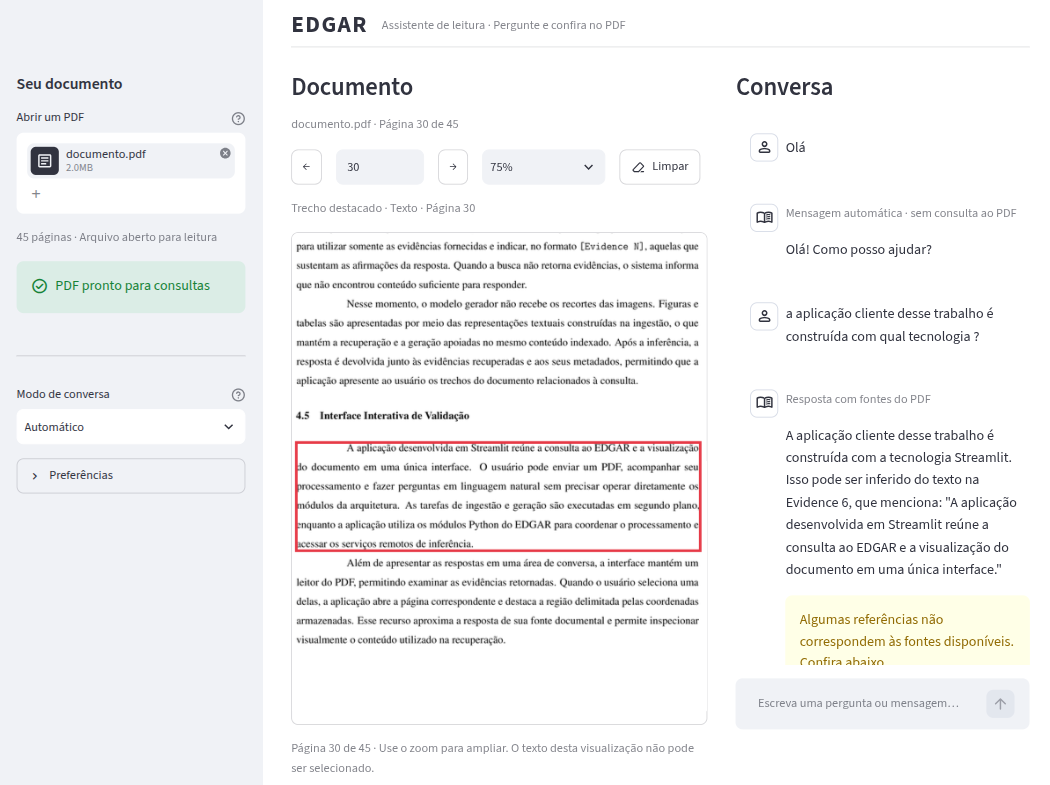
\includegraphics[width=0.88\textwidth,height=0.68\textheight,keepaspectratio]{figuras/evidencia_aplicacao_cliente.png}
    \legend{Fonte: Elaborado pelo autor.}
\end{figure}

\section{Discussão dos resultados e limitações}
\label{sec:discussao-resultados}

A análise qualitativa das respostas mostra tanto o benefício quanto o risco de converter elementos visuais em descrições textuais durante a ingestão. Na consulta sobre assíntota vertical em Cálculo, por exemplo, a descrição produzida pelo modelo de visão fez a página da figura subir da sexta posição em E3 para a primeira em E4, permitindo responder corretamente à pergunta. Em contrapartida, na consulta sobre frequência angular em Física, o modelo visual transcreveu incorretamente a relação \(\omega = 1/T\) a partir de uma figura que exibia \(\omega = 2\pi/T\). Como o modelo gerador fundamenta-se exclusivamente no texto recebido, ele reproduziu \(\omega = 1/T\) na resposta. Nesse tipo de situação, a resposta concorda com a evidência textual fornecida ao gerador, mas diverge do documento original, tornando o destaque visual da região (\textit{bbox}) no PDF indispensável para que o estudante confira a fonte e perceba o erro.

De modo complementar, o desempenho competitivo de E1 na busca de páginas (19/21) e nas perguntas de fórmulas (5,33/6) mostra que fragmentos de 1.000 caracteres com sobreposição preservam o contexto textual imediato ao redor de equações isoladas, que não receberam registros independentes no fluxo atual do EDGAR. Já quando a pergunta exige interpretar gráficos ou combinar mais de um componente dentro do limite de 5.000 unidades de entrada, a granularidade fina com descrição visual (E4) reduz o ruído contextual e alcança a maior média de qualidade das respostas (5,24/6).

Por fim, a interpretação desses achados deve considerar as limitações do estudo: (i) a restrição de créditos na plataforma Modal limitou o processamento a 500 páginas e a avaliação final a 21 consultas (com apenas três de Estatística); (ii) a comparação entre E3 e E4 reflete o efeito conjunto das mudanças no índice, na ordem da busca e no contexto entregue ao gerador; (iii) o gabarito verifica o documento e a página, e não o identificador individual de cada caixa delimitadora; e (iv) tanto a avaliação por critérios de qualidade (Codex) quanto o RAGAS (Qwen2.5-7B-Instruct, com 47 notas ausentes por truncamento) utilizaram avaliadores baseados em modelos de linguagem, sem etapa de validação humana independente.
